\let\negmedspace\undefined
\let\negthickspace\undefined
\documentclass[journal]{IEEEtran}
\usepackage[a5paper, margin=10mm, onecolumn]{geometry}
\usepackage{lmodern} % Ensure lmodern is loaded for pdflatex
\usepackage{tfrupee} % Include tfrupee package

\setlength{\headheight}{1cm} % Set the height of the header box
\setlength{\headsep}{0mm}     % Set the distance between the header box and the top of the text

\usepackage{gvv-book}
\usepackage{gvv}
\usepackage{cite}
\usepackage{amsmath,amssymb,amsfonts,amsthm}
\usepackage{algorithmic}
\usepackage{graphicx}
\usepackage{textcomp}
\usepackage{xcolor}
\usepackage{txfonts}
\usepackage{listings}
\usepackage{enumitem}
\usepackage{mathtools}
\usepackage{gensymb}
\usepackage{comment}
\usepackage[breaklinks=true]{hyperref}
\usepackage{tkz-euclide} 
\usepackage{listings}
 \usepackage{gvv}                                        
\def\inputGnumericTable{}                                 
\usepackage[latin1]{inputenc}                                
\usepackage{color}                                            
\usepackage{array}                                            
\usepackage{longtable}                                       
\usepackage{calc}                                             
\usepackage{multirow}                                         
\usepackage{hhline}                                           
\usepackage{ifthen}                                           
\usepackage{lscape}

\begin{document}

\bibliographystyle{IEEEtran}


\title{4.10.23}
\author{EE25BTECH11021 - Dhanush Sagar}

{\let\newpage\relax\maketitle}

\renewcommand{\thefigure}{\theenumi}
\renewcommand{\thetable}{\theenumi}
\setlength{\intextsep}{10pt} % Space between text and floats
\numberwithin{equation}{enumi}
\numberwithin{figure}{enumi}
\renewcommand{\thetable}{\theenumi}
\textbf{Question} \\

A straight the through a fixed point (2, 3) intersects the coordinate axes at distinct
points P and Q. If O is the origin and the rectangle OPRQ is completed, then the
locus of R is 

\textbf{Solution} \\
% --- Step 1: Equation of line through fixed point ---
\text{Equation of a line with normal vector $\vec{n}$ through } \myvec{2\\3}:
\begin{align}
\vec{n}^T\vec{x} &= \vec{n}^T\myvec{2\\3}  
\end{align}

% --- Step 2: Intercepts with axes ---
\text{The $x$-intercept is} $\vec{P}=\myvec{p\\0}$.
\text{The $y$-intercept is} $\vec{Q}=\myvec{0\\q}$. \\


% --- Step 3: Vertices of the rectangle ---
\text{The origin is}
\begin{align}
\vec{O} &= \myvec{0\\0}  
\end{align}



% --- Step 2: Relate u to the intercepts P and Q ---

\text{If the intercepts are } $\vec{P}=\myvec{p\\0},\; \vec{Q}=\myvec{0\\q}$, \text{ then normal vector is } 
\begin{align}
\vec{n} &= \myvec{\tfrac{1}{p}\\[3pt]\tfrac{1}{q}}
\end{align}

% --- Step 3: Opposite vertex R of rectangle OPRQ ---
\text{The opposite vertex of rectangle OPRQ is then } 
\begin{align}
\vec{R} &= \myvec{p\\[3pt]q}
\end{align}

% --- Step 4: Express the condition u^T(2,3)=1 in terms of R ---
\text{Write } $\vec{n}$ \text{ in terms of } $\vec{R}$ \text{ by }
\begin{align}
\vec{n}=\myvec{\tfrac{1}{p}\\[3pt]\tfrac{1}{q}}=\myvec{\tfrac{1}{x}\\[3pt]\tfrac{1}{y}}\text{ where } \vec{R}=\myvec{x\\y}:
\end{align}
\begin{align}
\myvec{\tfrac{1}{x} & \tfrac{1}{y}}\myvec{2\\3} &= 1
\end{align}

% --- Step 5: Multiply out and clear denominators to obtain locus ---
\text{Multiply out the left-hand side:}
\begin{align}
\tfrac{2}{x} + \tfrac{3}{y} &= 1
\end{align}

\text{Clear denominators by multiplying both sides by } xy:
\begin{align}
2y + 3x &= xy
\end{align}

\text{Rearrange to standard quadratic form:}
\begin{align}
xy - 3x - 2y &= 0
\end{align}

% --- Step 7: Expressing in quadratic form ---
\text{A conic in matrix form is } 
\begin{align}
\vec{x}^T \vec{V} \vec{x} + 2 \vec{u}^T \vec{x} + f = 0, \quad \vec{x} = \myvec{x\\y}.
\end{align}
\text{Here, the matrix corresponding to the } xy \text{ term is symmetric:}
\begin{align}
\vec{V} &= \myvec{0 & \tfrac{1}{2} \\[1mm] \tfrac{1}{2} & 0}, \quad
\vec{u} = \myvec{-3\\-2}, \quad f = 0
\end{align}

% --- Step 7: Final locus in matrix form ---
\begin{align}
\vec{x}^T \myvec{0 & \tfrac{1}{2} \\[1mm] \tfrac{1}{2} & 0} \vec{x} + 2 \myvec{-3\\-2}^T \vec{x} &= 0
\end{align}
\begin{figure}[H]
    \centering
    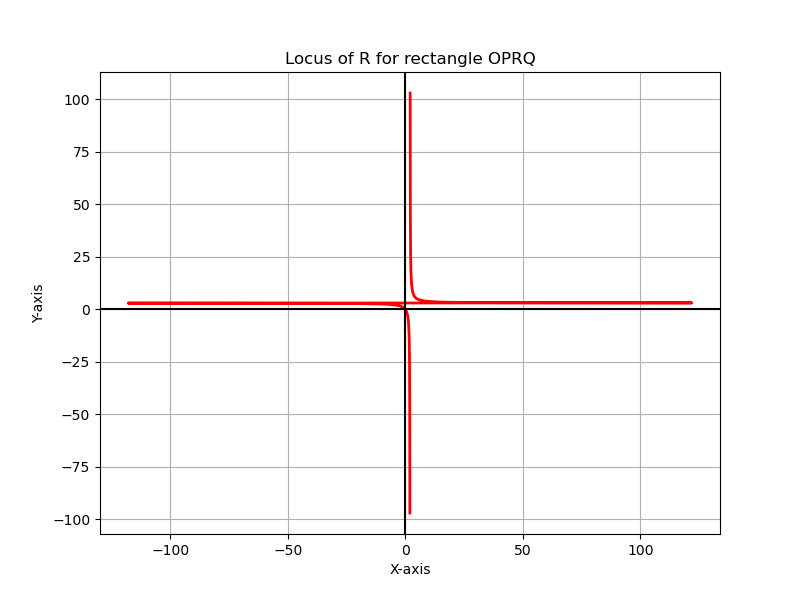
\includegraphics[width=0.5\columnwidth]{figs/fig1.png}
    \caption{}
    \label{fig:placeholder}
\end{figure}
\end{document}


% --- Step 1: Equation of line through fixed point ---
